\section{Harris corner detection}\label{P2}

TThe Harris Corner Detector is a well-known algorithm that is utilized for the purpose of locating corners or spots of interest within an image. The primary objective of the Harris Corner Detector is to identify substantial variations in intensity that occur in a variety of directions within a local neighborhood of a picture. There are points in the image when the intensity of the image suddenly changes in many directions, and these are known as corners. A structure tensor, which is a matrix that summarizes the local picture structure based on the image derivatives, might be constructed for each pixel in the image. This would allow us to construct a structure tensor. This is the formula for the structural tensor:


\[
M = \sum_{x, y} W(x, y)
\begin{bmatrix}
I_x I_x & I_x I_y \\
I_x I_y & I_y I_y
\end{bmatrix}
\]

Utilizing the determinant and trace of the structure tensor, the following steps can be taken to compute a corner response function:


\[
R = \det(M) - \alpha \cdot \operatorname{trace}^2(M)
\]

Additionally, the parameter $\alpha$ is a constant that is used to alter the sensitivity of the detector, which typically falls between the range of 0.04 to 0.06. When it comes to this particular exercise, the value that is deemed to be between these two numbers is 0.05. When analyzing the image, the corners are determined by the scores that are more than 0.3 of the maximum value of the R matrix. By adjusting this value, we are able to determine the total number of points that can be classified as the corner. The partial derivatives of the image are depicted in Figure 9, and the Gaussian filter is depicted in Figure 10.\\


\begin{figure}[h]
    \centering
    \begin{subfigure}{0.4\textwidth}
        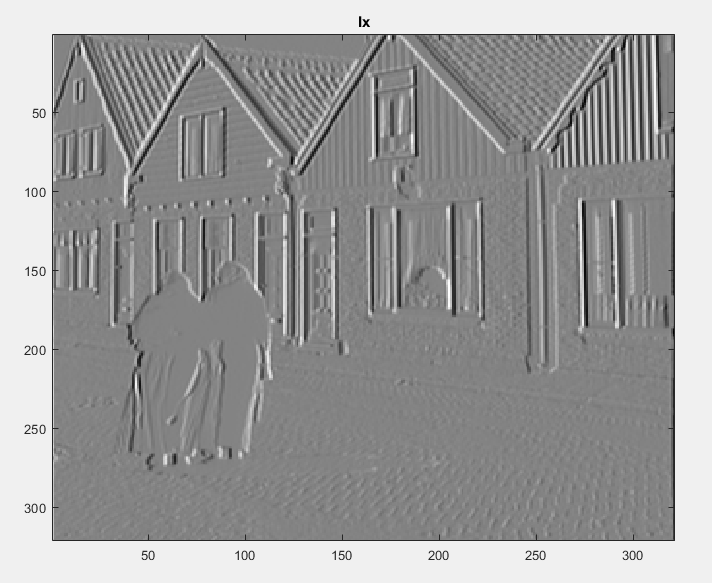
\includegraphics[width=\textwidth]{Resources/F9-1.PNG}
        \caption{}
        \label{fig:IX}
    \end{subfigure}
    \hfill
    \begin{subfigure}{0.4\textwidth}
        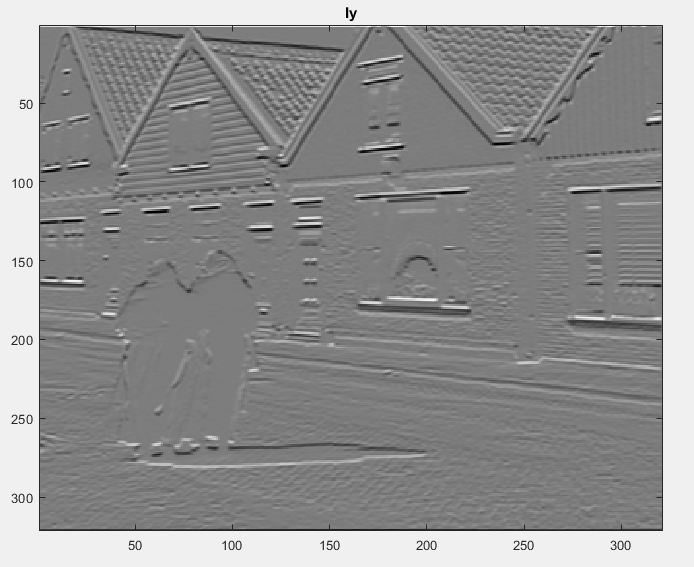
\includegraphics[width=\textwidth]{Resources/F9-2.png}
        \caption{}
        \label{fig:IY}
    \end{subfigure}
    \caption{The partial derivatives of the image}
    \label{fig:The partial derivatives of the image}
\end{figure}

\begin{figure} [ht]
    \centering
    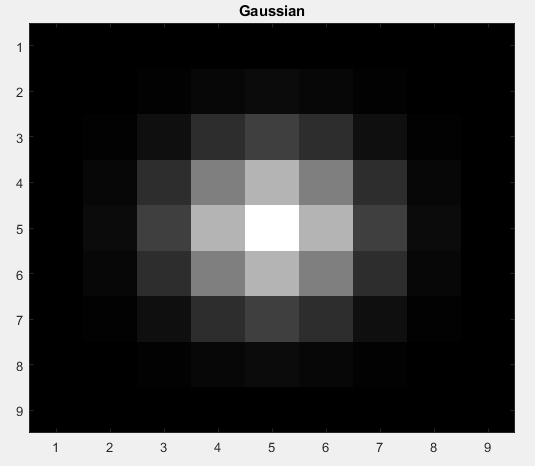
\includegraphics[width = 0.4\textwidth]{Resources/F10.png}
    \caption{The Gaussian filer}
    \label{fig:The Gaussian filer}
\end{figure}


\begin{figure} [ht]
    \centering
    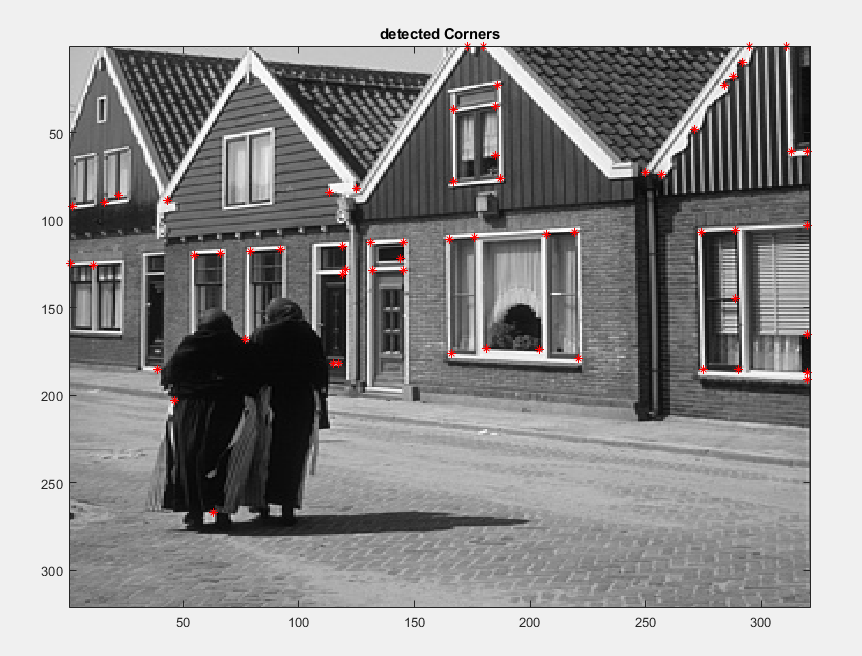
\includegraphics[width = \textwidth]{Resources/F11.png}
    \caption{The detected corners}
    \label{fig:The detected corners}
\end{figure}


There are three functions inside of the files that have been provided for the assignment. "Template Matching" is the name of the function that is responsible for fitting templates together. The function known as "ColorBased Segmentation" also performs a simulation of the color-based segmentation approach on the displayed images. The corner detection functionality is applied to the image by utilizing the Harris Corner() function. Every one of these routines is written in a separate file that is referred to as "main." You have the option of commenting out each function in the event that you do not require the results pertaining to that particular aspect of the problem.
